\documentclass{stdlocal}
\begin{document}
\section{Physical Simulations and Monte Carlo Methods} % (fold)
\label{sub:simulation_in_physics_and_mathematics}
  For our purposes, it is enough to explain the application of PRNGs to some given simulation procedures because there is no generic approach on how to randomize an arbitrary physical problem.
  Hence, we will not provide an excessive explanation to the theory of Monte Carlo methods and their application to general physical problems.
  Instead, the focus lies on the understanding of basic concepts and their implementation with respect to well-chosen examples.

  As mentioned in the introduction, section \ref{sec:introduction}, the simulation of physical and mathematical systems can be quite time intensive.
  Many degrees of freedom in a resulting partial differential equation make the problem infeasible to solve deterministically \autocite{landau2014}.
  This is typically called the \enquote{curse of dimensionality} \autocite{mueller2012}.
  As a consequence, we rely on probability theory to estimate the respective solutions and speed-up the simulation.
  Such randomized algorithms are in general called Monte Carlo methods \autocite{mueller2012,landau2014}.

  \begin{definition}[Monte Carlo Method]
    % A Monte Carlo method is an algorithm that uses the realization of random variables, also called random samples, to generate its result.
    A Monte Carlo method is a random variable that computes its result based on given random variables according to an algorithm.
    We call the realization of a Monte Carlo method a run or its execution.
  \end{definition}
  We will not give a rigorous definition of an algorithm but refer to \textcite{hromkovic2011} for detailed information.
  With this definition, the output of an execution of a Monte Carlo method is interpreted as a realization of random variables.
  In contrast to a deterministic algorithm, calling a Monte Carlo method twice with identical input arguments will not necessarily produce the same output again.
  This behavior lets them overcome the \enquote{curse of dimensionality} and as a result they represent an efficient family of generalized algorithms to solve high-dimensional problems.

  To get the idea behind Monte Carlo methods, the observation of direct simulations as given in \textcite{mueller2012} will serve perfectly.
  For some dimension $d\in\setNatural$, we want to approximate a value $r\in\setReal^d$ by a Monte Carlo method.
  Direct simulation needs an already existent sequence of iid random variables with their expectation value equal to $r$ which we interpret as random samples.
  But this does not impose strong restrictions because we are mostly able to find such random variables.

  \begin{lemma}[Direct Simulation]
    Let $d\in\setNatural$, $r\in\setReal^d$ and $(X_n)_{n\in\setNatural}$ a sequence of $\setReal^d$-valued iid random variables in $\setIntegrable^2\roundBrackets{\setReal^d,λ}$ with $\expect X_n = r$ for all $n\in\setNatural$.
    In this case, construct the following random variable for all $n\in\setNatural$.
    \[
      D_n \define \frac{1}{n}\sum_{k=1}^n X_k
    \]
    Then for arbitrary sample counts $n\in\setNatural$ the random variable $D_n$ is a Monte Carlo method which fulfills the following equations.
    \[
      \expect D_n = r
      % \separate
      % \var D_n = \frac{\var X_k}{n}
      \separate
      \stddev(D_n) = \frac{\stddev(X_1)}{\sqrt{n}}
      \separate
      \lim_{n\to\infty} \stddev(D_n) = 0
    \]
    % Using the SLLN, we get the following almost everywhere.
    Furthermore, the following limit holds almost everywhere.
    \[
      \lim_{n\to\infty} D_n = r
    \]
  \end{lemma}
  We will give no proof of this lemma and instead refer to \textcite{mueller2012}.
  Please note that the last limit follows from Theorem \ref{theorem:slln} the SLLN.
  The expectation value of the given method is always the result that we wanted to compute.
  This is not a special property.
  But looking at the standard deviation, the error of the direct simulation becomes smaller for a bigger sample count.
  Using a large number of samples will therefore estimate the actual result much more precisely.
  Additionally, the error is decreasing with $\frac{1}{\sqrt{n}}$.
  Hence, the error rate is independent of the given dimension which explains the overcoming of the \enquote{curse of dimensionality}.

  \subsection{Monte Carlo Integration and the Computation of $π$} % (fold)
  \label{sub:monte_carlo_integration}
    Many simulations involve the calculation of multidimensional integrals.
    As a consequence, the so-called Monte Carlo integration forms the natural application of the direct simulation.
    We want to estimate the integral of a function.
    For given uniformly distributed random variables, we will construct a sequence of random variables such that their expectation value will coincide with the integral.
    \autocite{mueller2012}

    \begin{definition}[Monte Carlo Integration]
    \label{definition:monte-carlo-integration}
      Let $d\in\setNatural$ be the dimension, $U\subset\setReal^d$ be a measurable and bounded subset, such that $0 < λ(U) < \infty$, and $f\in\setIntegrable^2(U,λ)$ the function to be integrated.
      Furthermore, let $(X_n)_{n\in\setNatural}$ be a sequence of iid, $U$-valued, and uniformly distributed random variables.
      Then the Monte Carlo integration of $f$ with $n$ samples on the domain $U$ is given by the following expression.
      \[
        \mathrm{MCI}_n(f) \define \frac{λ(U)}{n} \sum_{k=1}^n f\circ X_k
      \]
    \end{definition}
    The domain of definition has to be restricted so that the method has a chance of reducing the overall estimation error.
    Additionally, the function $f$ should be square-integrable such that we are able to get an upper bound on the standard deviation.
    The following lemma will show that Monte Carlo integration is indeed a Monte Carlo method with the properties of a direct simulation.
    \autocite{mueller2012}

    \begin{lemma}[Monte Carlo Integration Estimates Value of Integral]
    \label{lemma:monte-carlo-integration}
      Choose the same setting as in the above definition \ref{definition:monte-carlo-integration}.
      In this case for all $n\in\setNatural$, the Monte Carlo integration $\mathrm{MCI}_n(f)$ is a Monte Carlo method and the following statements for the expectation value and standard deviation are fulfilled.
      \[
        \expect \mathrm{MCI}_n(f) = \integral{U}{}{f}{λ}
        \separate
        \stddev\boxBrackets{\mathrm{MCI}_n(f)} \leq \sqrt{\frac{λ(U)}{n} \integral{U}{}{f^2}{λ}}
      \]
    \end{lemma}
    % \begin{proof}[Lemma \ref{lemma:monte-carlo-integration} on page \pageref{lemma:monte-carlo-integration}]
    %   Let $p$ be the probability density of $X_n$.
    %   Because the random variables are uniformly distributed on $U$, we can express it as follows.
    %   \[
    %     \function{p}{U}{[0,\infty)}
    %     \separate
    %     p(x) \define \frac{1}{λ(U)}
    %   \]
    %   By using substitution and chaining from propositions \ref{proposition:substitution} and \ref{proposition:chaining}, the expectation value can be directly computed.
    %   \[
    %     \begin{aligned}[t]
    %       \expect \mathrm{MCI}_n(f)
    %       &= \expect \boxBrackets{ \frac{λ(U)}{n} \sum_{k=1}^n f\circ X_k }
    %       = \frac{λ(U)}{n} \sum_{k=1}^n \expect(f\circ X_k) \\
    %       &= λ(U) \integral{U}{}{f(x) p(x)}{λ(x)}
    %       = \integral{U}{}{f}{λ}
    %     \end{aligned}
    %   \]
    %   For the standard deviation, first the variance will be observed.
    %   Since the sequence of random variables is stochastically independent, the sum can be taken out of the argument.
    %   Afterwards, we again apply substitution and chaining.
    %   \[
    %     \begin{aligned}
    %       \var \mathrm{MCI}_n(f) &= \var\boxBrackets{ \frac{λ(U)}{n} \sum_{k=1}^n f\circ X_k } = \frac{λ(U)^2}{n^2} \sum_{k=1}^n \var\roundBrackets{f\circ X_k} \\
    %       &= \frac{λ(U)^2}{n^2} \sum_{k=1}^n \expect\roundBrackets{f\circ X_k}^2 - \boxBrackets{\expect\roundBrackets{f\circ X_k}}^2 \\
    %       &\leq \frac{λ(U)^2}{n^2} \sum_{k=1}^n \expect\roundBrackets{f\circ X_k}^2 = \frac{λ(U)^2}{n} \integral{U}{}{f^2(x) p(x)}{λ(x)} \\
    %       &= \frac{λ(U)}{n} \integral{U}{}{f^2}{λ}
    %     \end{aligned}
    %   \]
    %   The inequality is now inferred by the definition of the standard deviation which proofs the lemma.
    %   \[
    %     \stddev\boxBrackets{\mathrm{MCI}_n(f)} = \sqrt{\var \mathrm{MCI}_n(f)} \leq \sqrt{\frac{λ(U)}{n} \integral{U}{}{f^2}{λ}}
    %   \]
    % \end{proof}
    In the proof, seen in appendix \ref{sec:proofs}, we basically applied the lemma about the direct simulation.
    So we get the same convergence rate for the expectation value with respect to the standard deviation.
    To get a deeper understanding of this method, consider the estimation of $π$ by Monte Carlo integration.
    For this, we would like to compute the area of a quarter of a circle which is strongly related to π.
    Figure \ref{fig:pi-computation-points} shows the execution of the following process for different realizations.


    \begin{figure}
      \center
      \begin{subfigure}[b]{0.32\linewidth}
        \center
        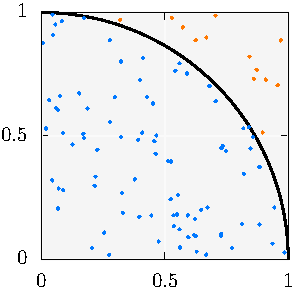
\includegraphics[width=\linewidth]{../../../examples/monte_carlo_pi_100_87.pdf}
        \caption{%
          \quad
          \begin{minipage}[t]{0.5\linewidth}
            $n = 100$ \\
            $s = 87$ \\
            $μ = 3.48$ \\
            $ε \approx 1.07 \cdot 10^{-1}$
          \end{minipage}
        }
      \end{subfigure}
      \hfill
      \begin{subfigure}[b]{0.32\linewidth}
        \center
        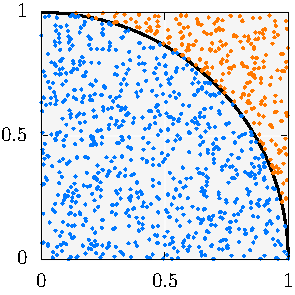
\includegraphics[width=\linewidth]{../../../examples/monte_carlo_pi_1000_765.pdf}
        \caption{%
          \quad
          \begin{minipage}[t]{0.5\linewidth}
            $n = 1000$ \\
            $s = 765$ \\
            $μ = 3.06$ \\
            $ε \approx 2.60 \cdot 10^{-2}$
          \end{minipage}
        }
      \end{subfigure}
      \hfill
      \begin{subfigure}[b]{0.32\linewidth}
        \center
        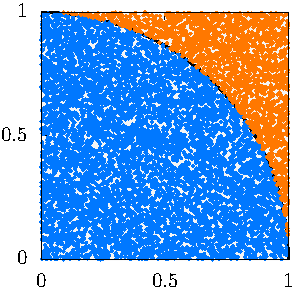
\includegraphics[width=\linewidth]{../../../examples/monte_carlo_pi_10000_7856.pdf}
        \caption{%
          \quad
          \begin{minipage}[t]{0.5\linewidth}
            $n = 10000$ \\
            $s = 7856$ \\
            $μ = 3.1424$ \\
            $ε \approx 2.57 \cdot 10^{-4}$
          \end{minipage}
        }
      \end{subfigure}
      \caption[Monte Carlo Integration and the Computation of π]{%
        Sample points for different realizations of the Monte Carlo integration $\mathrm{MCI}_n(f)$ for the computation of π.
        Points that lie in the quarter of the unit circle are shown in blue color whereas other points are shown in orange color.
        The unit circle is represented by a black line.
        The result of the realizations is expressed by the sample mean μ and the relative error with respect to π is expressed by ε.
        The variable $s$ names the count of samples that lie in the unit circle.
      }
      \label{fig:pi-computation-points}
    \end{figure}

    Computing the area of a subset is in general done by integration.
    Therefore we choose $d=2$ and $U\define [0,1]^2$ with $λ(U) = 1$.
    Thus, the random variable $X_n$ will be uniformly distributed on $[0,1]^2$ for all $n\in\setNatural$.
    The last part consists of the construction of the function $f$.
    First, define the set which characterizes the quarter of the unit circle.
    \[
      G \define \set{x \in [0,1]^2}{\norm{x} \leq 1}
      \separate
      λ(G) = \frac{π}{4}
    \]
    Based on this set, the function $f$ can be expressed through the use of the characteristic function of $G$ and by scaling its value.
    \[
      f \define 4\cdot\mathds{1}_G
      \separate
      \expect \mathrm{MCI}_n(f) = \integral{U}{}{f}{λ} = 4 \integral{[0,1]^2}{}{\mathds{1}_G}{λ} = 4\cdotλ(G) = π
    \]
    Simulating the integral of $f$ will therefore give us an estimation of π.
    For a more detailed analysis, we will also compute the exact standard deviation of this Monte Carlo integration by using the above lemma \ref{lemma:monte-carlo-integration}.
    \[
      \integral{U}{}{f^2}{λ} = 16 \integral{[0,1]^2}{}{\mathds{1}_G}{λ} = 16\cdot λ(G) = 4π
    \]
    \[
      \begin{aligned}
        \var\roundBrackets{f\circ X_1}
        &= \expect\roundBrackets{f\circ X_1}^2 - \boxBrackets{\expect\roundBrackets{f\circ X_1}}^2
        = \integral{U}{}{f^2}{λ} - \roundBrackets{\integral{U}{}{f}{λ}}^2 \\
        &= 4π - π^2 = π(4-π)
      \end{aligned}
    \]
    \[
      \stddev\roundBrackets{\mathrm{MCI}_n(f)} = \sqrt{\frac{π(4-π)}{n}} \leq 2\sqrt{\frac{π}{n}} = \sqrt{\frac{λ(U)}{n} \integral{U}{}{f^2}{λ}}
    \]
    In figure \ref{fig:pi-computation-plots}, we can see this behavior for some actual simulations.
    By taking a larger amount of samples, the volume of the quarter of the unit circle becomes more occupied as can be seen in figure \ref{fig:pi-computation-points}.
    As a consequence, the estimation of π will be more precise.
    Furthermore, figure \ref{fig:pi-computation-plots} shows that the error of the estimation can also be estimated and will be more precise for a larger sample count.
    \autocite{mueller2012,landau2014,pharr2016}

    \begin{figure}
      \center
      \begin{subfigure}[b]{0.49\linewidth}
        \center
        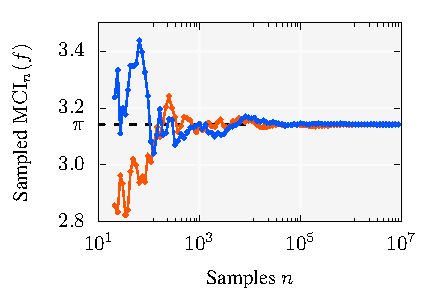
\includegraphics[width=\linewidth]{../../../examples/monte_carlo_pi_plot.pdf}
      \end{subfigure}
      \begin{subfigure}[b]{0.49\linewidth}
        \center
        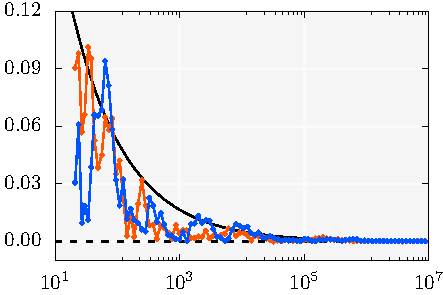
\includegraphics[width=\linewidth]{../../../examples/monte_carlo_pi_plot_error.pdf}
      \end{subfigure}
      \caption[Monte Carlo Integration Plots for the Computation of π]{%
        Each of the diagram shows two different versions, colored in orange and blue, of realizations of the Monte Carlo integration $\mathrm{MCI}_n(f)$ for the computation of π for different values of $n$.
        The left one displays the estimated value of π and the right one displays its relative error with respect to π.
        The black line hereby shows the exact relative standard deviation with respect to π of the Monte Carlo integration.
      }
      \label{fig:pi-computation-plots}
    \end{figure}

    Later, we will use the computation of π as benchmark routine to measure the performance of PRNGs with respect to different aspects of their implementation.
    In these cases, the error of π should be in some given range.
    Assume we want to use $10^8$ samples to estimate the value of π.
    According to the formula above for the standard deviation, we get an error of approximately $0.00016$ which means we should at least get a precision of four digits, such that π should approach the value $3.1415$ with a varying last digit.

    To use the described Monte Carlo integration for estimating π, an actual implementation in C++ is needed.
    The following code snippet provides the basic algorithm relying on the random utilities given by the STL of the C++ programming language.
    Because C++ is a strongly typed language which is working with templates for type abstraction, the given code uses templates to generalize the usage of different RNG types, as well as different real and integer number types.
    Typically, we will use the \code{float} type as the real number type and the \code{int} type as the integer type.

    \inputCodeBlock[title=Basic Monte Carlo π Computation]{code/monte_carlo_pi.hpp}
    The implementation of the algorithm does not introduce any irregularities and can directly be deduced from the mathematical formulation.
    First, we define the standard uniform distribution for the RNG and an integer number \code{samples\_in\_circle} as zero which will be used to count the number of samples that lie inside the unit circle.
    In the following \code{for} loop every run will construct two uniformly distributed random numbers which together will define the position of a random two-dimensional point in the unit square.
    We then evaluate the circle condition and add its result to \code{samples\_in\_circle} incrementing it by one if the condition is true and by zero otherwise.
    At the end, the code computes the correct result by calculating the division and scaling the output.

    % The application of the given library function is shown in the following source file.
    % \inputCodeBlock[title=monte\_carlo\_pi.cpp]{code/monte_carlo_pi.cpp}

    The computation of π is only an academic example that should not be used in reality because there are much more efficient ways to estimate it.
    But as we will see, it is perfectly suited as a benchmark to test different kinds of RNGs because the main part of the algorithm consists of generating a lot of random numbers while using their values to actually compute a result.
    Evaluating the circle condition for generated random numbers is fast and will not introduce a lot of bias in the actual measurement.
    Besides, it is the most common example of a non-trivial Monte Carlo integration.
    A lot of physical problems rely on Monte Carlo integration.
    In the end, all these problems can be broken down into similar forms as the computation of π.
    \autocite{mueller2012,landau2014,pharr2016}
  % subsection monte_carlo_integration_and_the_computation_of_ (end)

  % \subsection{Metropolis-Hastings Algorithm and the Ising Model} % (fold)
  % \label{sub:metropolis_hastings_algorithm_and_the_ising_model}

  % subsection metropolis_hastings_algorithm_and_the_ising_model (end)

  \subsection{Photon Propagation and Physically Based Rendering} % (fold)
  \label{sub:photon_propagation_and_physically_based_rendering}
    A photon is an elementary particle and the quantum of the electromagnetic field.
    It exhibits properties of both waves, like wavelength and polarization, and particles, such as position and momentum.
    This is also known as wave-particle duality.
    In vacuum, photons always move at the speed of light.
    Their invariant mass is zero and therefore they are thought of as massless particles.
    Due to Heisenberg's uncertainty principle, we are in general not able to measure their position and momentum at the same time with infinite precision.
    Because we are concerned about the photon propagation in space at a large scale, we will use an abstract concept of a photon to approximate physical laws and making simulations feasible.
    We think of an abstract photon as a packet of photons with a definite position and velocity representing their respective expectation values of all the photons inside the packet.
    Since the positions and velocities are then based on statistical calculations, this will allow us to ignore the uncertainty principle.
    Additionally, we assume no particular polarization or wavelength in the packet can be determined.
    Thus, the wavelength will be ignored and the abstract photon will be seen as unpolarized.

    In computer graphics, the rendering of realistic images based on physical principles requires the simulation of global illumination effects.
    Global illumination is formally described by the so-called rendering equation, also known as light transport equation (LTE).
    There exist several different formulations of the LTE, such as the surface form and the path integral formulation, which are all equivalent and are used to derive advanced methods to actually estimate the light distribution in space consisting of differing objects.
    The LTE can be derived by applying principles of geometric optics to the law of the conservation of energy for electromagnetic radiation.
    A detailed explanation is given in \textcite{pharr2016} and a mathematically rigorous discussion can be read in \textcite{pawellek2017}.

    \begin{figure}
      \center
      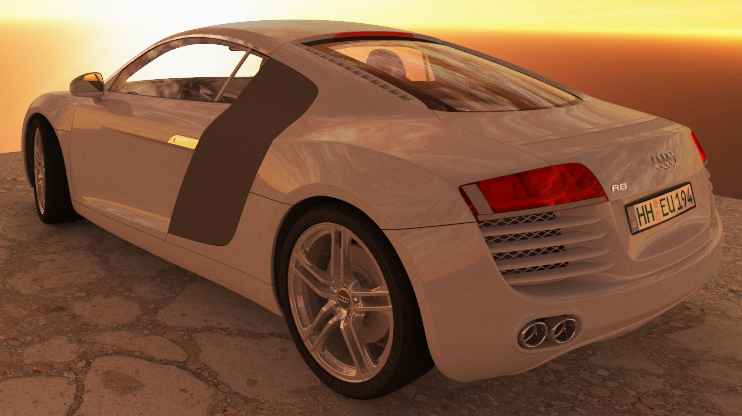
\includegraphics[width=0.9\textwidth]{images/audi_r8_path_tracing.png}
      \caption[Path Tracing Example]{%
        Example scene showing an Audi R8 rendered by the path tracing algorithm.
        The simulation included ideal reflections and refractions, as well as the diffuse scattering of light at the surfaces.
        The simulation used $1024$ samples per pixel to reduce the noise of the image.
        \autocite{pawellek2017}
      }
      \label{fig:path-tracing-r8}
    \end{figure}

    Typically, the LTE cannot be evaluated analytically for complex geometries.
    As a consequence, there are multiple famous simulation strategies, like path tracing, bidirectional path tracing, metropolis light transport, and photon mapping, to approximate its solutions.
    All of these strategies have in common that they are somehow estimating the light distribution in space through Monte Carlo methods.
    Because of the integral appearing inside the equation, all algorithms make great use of Monte Carlo integration in different ways.
    Path tracing, for example, is using the path integral formulation of the LTE by importance sampling different paths of light through the scene starting from the observer and ending at a light source.
    At every vertex of the path, \enquote{Russian roulette} decides if the ray has to be reflected, transmitted or absorbed.
    In general, the algorithm has to compute several hundreds of sample paths for every pixel on the screen to reduce the noise and get an acceptable estimation  of the actual light distribution.
    Figure \ref{fig:path-tracing-r8} shows an example scene rendered by the path tracing algorithm for which more than a thousand samples per pixel had to be generated.
    As a consequence, the tracing of rays and the propagation of photons through a scene needs to use a really large amount of random numbers.
    \autocite{pharr2016}

    The tracing of light rays is strongly connected to photon propagation in space.
    From an abstract point of view, we can think of light rays as packets of photons.
    Light rays are used to gather the radiance arriving at the observer whereas photons propagate flux from a light source.
    At large scale, both of them adhere to the same laws even if they are interpreted differently.
    Hence, photon tracing works exactly the same way as ray tracing.
    A usual application of this phenomenon is the photon mapping algorithm.
    The movement and transmission of differing photons or rays does not depend on each other.
    Due to the high amount of random numbers needed and the large degree of independence, the simulation of global illumination by using Monte Carlo methods seems to be convenient to measure the performance improvement by applying vectorized PRNGs.
    This claim is even supported by an already existing strong usage of SIMD instructions for the current most efficient ray and path tracing engines \autocite{embree}.

    In this thesis, it is not possible to provide a complete ray tracing framework to test the application of vectorized PRNGs.
    But we are able to construct a simplified version which is using the developed PRNGs to simulate the propagation of photons.
    This smaller simulation focuses on the most important physical effects and ignores subtleties that would introduce bias in the performance measurements.
    We will provide the physical background concerning photon propagation.

    % \begin{definition}[Photon]

    % \end{definition}

    % \subsubsection*{Surface Interaction} % (fold)
    % \label{ssub:surface_interaction}
    %   The interaction of photons with surfaces of objects is strongly associated with the properties of the materials the objects consist of.
    %   Typically, the behavior can be modeled by bidirectional scattering distribution functions (BSDFs) which give the portion of light scattered in the outgoing direction with respect to the incoming direction.
    %   Concerning photons, for a fixed incoming direction BSDFs can be thought of as probability densities over the outgoing direction of the photon after the surface scattering has taken place.
    %   We refer again to \textcite{pharr2016} and \textcite{pawellek2017}.
    %   To simulate complex optical properties of object materials BSDFs have to be sampled with the usage of appropriate random variables.
    %   In this context, we will only assume ideal reflection and refraction of photons to not introduce unnecessary complexness to the application.

    %   \begin{figure}
    %     \center
    %     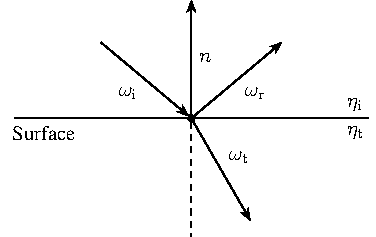
\includegraphics[height=0.3\textwidth]{figures/reflection_refraction_scheme.pdf}
    %     \caption[Ideal Reflection and Refraction]{%
    %       Ideal reflection and refraction scheme and notation.
    %       The surface with surface normal $n$ separates the outer medium with refractive index $η_\mathrm{i}$ from the inner medium with refractive index $η_\mathrm{t}$.
    %       $ω_\mathrm{i}$, $ω_\mathrm{r}$, and $ω_\mathrm{t}$ denote the incoming, reflection, and refraction direction, respectively.
    %     }
    %     \label{fig:reflection-refraction-scheme}
    %   \end{figure}

    %   Ideal reflection of a photon means that the angle between its incoming direction and the surface normal is the same as the angle between the outgoing direction and the surface normal.
    %   In general, we can define it as follows.

    %   \begin{definition}[Ideal Reflection]
    %     For any incoming direction $ω_\mathrm{i}\in \mathscr{S}^2$ its ideally reflected direction $ω_\mathrm{r}$ with respect to a surface with surface normal $n\in\mathscr{S}^2$ is given by the following equation.
    %     \[
    %       ω_\mathrm{r} = ω_\mathrm{i} - 2 \scalarProduct{n}{ω_\mathrm{i}} n
    %     \]
    %   \end{definition}
    %   A refractive index is a dimensionless number and represents the slow-down in speed when light is traveling through the according medium.
    %   The ideal refraction of photons traveling through a surface which is separating two media with varying refractive indices can be described by the following definition.

    %   \begin{definition}[Ideal Refraction]
    %     For any incoming direction $ω_\mathrm{i}\in \mathscr{S}^2$ its ideally refracted direction $ω_\mathrm{t}$ with respect to a surface with surface normal $n\in\mathscr{S}^2$ is given by the following equation.
    %     \[
    %       ω_\mathrm{t} =
    %       \begin{cases}
    %         \frac{η_\mathrm{i}}{η_\mathrm{t}} \roundBrackets{ ω_\mathrm{i} - \scalarProduct{n}{ω_\mathrm{i}} n} - \sqrt{ξ} n & :ξ > 0 \\
    %         ω_\mathrm{r} & :ξ \leq 0
    %       \end{cases}
    %     \]
    %     \[
    %       ξ \define \frac{η^2_\mathrm{i}}{η^2_\mathrm{t}}\roundBrackets{1 - \scalarProduct{n}{ω_\mathrm{i}}^2}
    %     \]
    %     Hereby, we assume that $ω_\mathrm{r}$ is the ideally reflected direction and that the surface is separating the outer medium with refractive index $η_\mathrm{i}\in [1,\infty)$ from the inner medium with refractive index $η_\mathrm{t}\in [1,\infty)$.%
    %   \end{definition}
    %   Figure \ref{fig:reflection-refraction-scheme} shows ideal reflection and refraction schematically.
    %   The connection between the angle of incidence and the angle of emergence is given by Snell's law.
    %   If the outer medium exhibits a larger refractive index than the inner medium then there exists a critical incident angle at which total reflection of the incoming photon occurs.
    %   This explains the distinction of cases in the above definition.
    %   Here, the second case represents total reflection.

    %   A photon can either be reflected or transmitted but not both at the same time.
    %   Hence, the surface coefficients $α,β\in [0,1]$ for reflection and refraction with $α+β=1$ of photons should be interpreted as probabilities.
    %   The interaction process can then be described by a probability density $p_{\omega_\mathrm{i}}$ over the outgoing directions $ω_\mathrm{o}\in \mathscr{S}^2$ with a fixed incoming direction $ω_\mathrm{i}\in\mathscr{S}^2$.
    %   In the case of ideal reflection $ω_\mathrm{r}$ and refraction $ω_\mathrm{t}$, we have
    %   \[
    %     p_{ω_\mathrm{i}}(ω_\mathrm{o}) \define α δ_{ω_\mathrm{o}}(ω_\mathrm{r}) + β δ_{ω_\mathrm{o}}(ω_\mathrm{t})
    %   \]
    %   where $δ_{ω_\mathrm{o}}$ denotes the Dirac delta distribution over $\mathscr{S}^2$.
    %   To sample the photon paths from such a probability density, Russian roulette is used to choose between reflection and refraction.

    %   \begin{lemma}[Russian Roulette]
    %     Choose the same settings as in definition \ref{definition:monte-carlo-integration}.
    %     Furthermore, assume $α,β\in [0,1]$ with $α+β=1$ and $f=αf_1 + βf_2$ for functions $f_1,f_2\in\mathrm{L}^2(U,λ)$.
    %     We define the roulette function $R$ as follows.
    %     \[
    %       \function{R}{[0,1]}{\set{1,2}{}}
    %       \separate
    %       R(x) \define
    %       \begin{cases}
    %         1 &: x \leq α \\
    %         2 &: \mathrm{else}
    %       \end{cases}
    %     \]
    %     In this case, for all $x\in U$ and $k\in\setNatural$ the following equation holds.
    %     \[
    %       f(x) = \expect f_{R\circ X_k} (x)
    %     \]
    %   \end{lemma}
    %   We will give no proof of this lemma.
    %   Russian roulette does not introduce any bias and allows us to only choose one path for the photon.
    %   This comes at the cost of a higher variance of the estimation.
    %   If we would evaluate both, reflection and refraction, at once and scale the results according to α and β then the estimation would have a variance of zero.
    %   But always tracing the possible paths soon becomes infeasible due to the exponential growth of different paths for every surface interaction.
    %   Russian roulette reduces this computational amount.
      % \[
      %   \mathrm{RR} \define \frac{λ(U)}{n} \sum_{k=1}^n f_{R(X_{2k})}\circ X_{2k-1}
      % \]
    % subsubsection surface_interaction (end)

    \subsubsection*{Volume Scattering} % (fold)
    \label{ssub:volume_scattering}
      Photons propagating through participating media are affected by absorption and scattering.
      Both processes are in general modeled by statistical processes.
      For our purpose, absorption will be ignored to reduce the complexity of the physical simulation.
      Scattering changes the direction of the photon.
      This process is described by rotation matrices and therefore scattering is much more appropriate for vectorization than absorption.
      \autocite{pharr2016}

      As a photon passes through a medium, it may collide with other particles and be scattered in different directions.
      The probability of a scattering event is modeled by the scattering coefficient which in our case equals to the extinction.
      We will only assume homogeneous media with a constant extinction.
      Hence, the actual probability of a scattering event after traveling a short distance is given by Beer's law.
      Because we want to show the application of RNGs to physical simulations, it is sufficient to directly define this probability without using the extinction.
      \autocite{pharr2016}

      Scattering itself is described by phase functions which are probability densities.
      Based on an incoming direction, they give the probability that the photon will be scattered in a certain outgoing direction.
      In this thesis, isotropic phase functions are used.
      They are invariant under rotations and therefore only depend on the angle between the incoming and outgoing direction.
      According to \textcite{pharr2016}, a widely used family of phase functions was developed by Henyey and Greenstein in the year 1941.
      This family cannot be deduced by physical laws but instead was specifically designed to be easy to fit to measured scattering data by only using a single parameter.
      \autocite{pharr2016,wang1995}

      \begin{definition}[Henyey-Greenstein Family of Phase Functions]
        Let $g\in [-1,1]$ be the asymmetry parameter, $ω_\mathrm{i}\in\mathscr{S}^2$ be the incoming direction of a photon and $ω_\mathrm{o}\in\mathscr{S}^2$ be a possible outgoing direction.
        The probability density $\function{p}{[-1,1]}{[0,\infty)}$ describing the distribution of $\cos ϑ \define \scalarProduct{ω_\mathrm{i}}{ω_\mathrm{o}}$ after a scattering process has taken place is then given by the following equation.
        \[
          p_g(\cos ϑ) \define \frac{1}{2} \frac{1-g^2}{(1+g^2 - 2g\cos ϑ)^{\frac{3}{2}}}
        \]
      \end{definition}
      To actually use the probability density $p_g$, we have to sample it.
      That means we have to construct a sequence of iid random variables with a distribution given by $p_g$.
      For this we will rely on a uniformly distributed sequence of iid random variables by applying a transformation to change their distribution.
      The following lemma can be shown by using the inversion method.
      A detailed derivation is given in \textcite{wang1995}.

      \newpage

      \begin{lemma}[Sampling Henyey-Greenstein Phase Functions]
        Let $g\in [-1,1]$ be the asymmetry parameter, $(X_n)_{n\in\setNatural}$ be a uniformly distributed sequence of iid random variables in the unit interval.
        Furthermore, let $(\cos ϑ_n)_{n\in\setNatural}$ be a sequence of random variables given by the following transformation.
        \[
          \cos ϑ_n =
          \begin{cases}
            \frac{1}{2g} \boxBrackets{1 + g^2 - \roundBrackets{\frac{1-g^2}{1-g+2gX_n}}^2} &: g\neq 0 \\
            2X_n - 1 &: g = 0
          \end{cases}
        \]
        Then, $(\cos ϑ_n)$ is a sequence of iid random variables distributed according to $p_g$.
      \end{lemma}
      The given lemma makes it possible to simulate scattering processes adhering to the probability density $p_g$ only by using uniformly distributed random numbers in the unit interval.

    % subsubsection volume_scattering (end)
  % subsection photon_propagation_and_physically_based_rendering (end)
% section simulation_in_physics_and_mathematics (end)
\end{document}